\documentclass[utf8]{frontiersSCNS}
\usepackage{gensymb}
\usepackage{url,hyperref,lineno,microtype,subcaption}
\usepackage[onehalfspacing]{setspace}

\linenumbers
\usepackage{wasysym} % provides \DH, \dh, \Thorn, \thorn
% Leave a blank\usepackage{amsmath}
%\DeclareMathOperator{\sign}{sign} line between paragraphs instead of using \\

\usepackage{booktabs}
\usepackage{multirow}
\usepackage{siunitx} %for SI units

\def\keyFont{\fontsize{8}{11}\helveticabold }
\def\firstAuthorLast{Balasubramanian {et~al.}} %use et al only if is more than 1 author
\def\Authors{Suryanarayanan Balasubramanian\,$^{1}$, Martin Hoelzle\,$^{1}$}
\def\Address{$^{1}$University of Fribourg, Department of Geosciences, Fribourg, Switzerland\\} \def\corrAuthor{Suryanarayanan Balasubramanian}

\def\corrEmail{suryanarayanan.balasubramanian@unifr.ch}


\begin{document}
\onecolumn
\firstpage{1}

\title[Artificial Ice Reservoirs]{Optimal discharge rates for artificial ice reservoir (Icestupa) evolution}

\author[\firstAuthorLast ]{\Authors}
\address{}
\correspondance{}

\extraAuth{}

% \maketitle
\begin{abstract}
  Since 2014, mountain communities in Ladakh, India have been constructing dozens of Artificial Ice Reservoirs
  (AIRs) by spraying water through fountain systems every winter. The meltwater from these structures is crucial
  to meet irrigation water demands during spring. However, the water use efficiency (WUE) of this technology is
  poor due to the variability of AIR freezing rates due to the weather and fountain influences at the chosen
  location. This study compares the WUE between an AIR constructed manually with an AIR constructed using
  automated systems at Guttannen, Switzerland. The automation software uses a simplified equation with 6
  coefficients that capture the influence of temperature, humidity, wind and solar radiation variations on the
  freezing rate. Historical meteorological data in conjunction with the coordinates, altitude and time zone of
  the site are required to calculate these 6 coefficients. The automated AIR had a WUE three times more
  than the manual AIR. This is a promising result for dry mountain regions, where automated AIR technology could
  scale current mitigation efforts.

	\tiny
	\keyFont{ \section{Keywords:} icestupa, water storage, climate change adaptation, geoengineering, nature based
  solution} %All article types: you may provide up to 8 keywords; at least 5 are mandatory.
\end{abstract}

\section{Introduction}

\section{Study Sites and data}

\section{Automation software}

The objective of the automation software is to estimate the optimal discharge rate given minimal weather,
fountain and location information. In order to do so, we simplify the methodology used in our previous paper
with some assumptions. We tend to use assumptions that overestimate the associated freezing rate to optimise
more for maximum ice volume rather than WUE. Below we present each of our assumptions corresponding to the
different model modules in our previous paper.

\subsection{Surface area calculation} \label{sec:shape}

The software approximates the area of the conical AIR to be equal to the area of its circular base. Therefore,
the surface area used

\begin{equation} A_{cone} =\pi \cdot r_{cone}^2 \label{eq:Area} \end{equation}

Admittedly, this assumption underestimates the surface area of the AIR during the accumulation period and
overestimates the surface area during the ablation period.  

\subsection{Energy balance calculation} \label{sec:energy}

We approximate the energy balance at the surface of an AIR by a one-dimensional description of energy fluxes as
used in \cite{Balasubramanian_2022}:

\begin{equation}
	 q_{freeze} + q_{melt} = q_{SW} + q_{LW} + q_{L} + q_{S}
	\label{eqn:EB}
\end{equation}

Upward and downward fluxes relative to the ice surface are positive and negative, respectively. The first two
terms represent the energy change used for freezing the fountain water and melting the ice respectively. The
third term represents the energy used for changing the surface temperature. $q_{SW}$ is the net shortwave
radiation; $q_{LW}$ is the net longwave radiation; $q_{L}$ and $q_{S}$ are the turbulent latent and sensible
heat fluxes.  Here, we define the surface temperature $T_{ice}$ to be the modelled average temperature of the
icestupa surface layer.

The software ignores $q_{T}$, $q_{F}$ and $q_{G}$. All these assumptions overestimate the freezing energy flux.

\subsubsection{Net Shortwave Radiation \texorpdfstring{$q_{SW}$}{Lg}} \label{sec:SW}

The net shortwave radiation $q_{SW}$ is computed as follows:

\begin{equation} q_{SW} = (1- \alpha_{ice})\cdot SW_{global} \label{eqn:SW} \end{equation}

where $\alpha_{ice}$ is the bare ice albedo value (0.25) and $SW_{global}$ is the global shortwave radiation.
The global shortwave radiation used is modelled using the parametrisation proposed by \cite{Woolf_1968}.

The software ignores (a) the differential absorption of $SW_{direct}$ and $SW_{diffuse}$ due to the conical
shape and (b) the variations in the albedo to simplify the model. Both these assumptions overestimate the solar
radiation thereby underestimating the freezing energy flux.

\subsubsection{Net Longwave Radiation \texorpdfstring{$q_{LW}$}{Lg}} \label{sec:LW}

The net longwave radiation $q_{LW}$ is determined as follows:

\begin{equation}
	q_{LW}= \sigma \cdot \epsilon_a \cdot {(T_a+ 273.15)}^4 -\sigma \cdot \epsilon_{ice} \cdot {(T_{ice}+ 273.15)}^4
	\label{eqn:LW}
\end{equation}

where $T_a$ represents the measured air temperature, $\epsilon_a$ denotes the atmospheric emissivity $T_{ice}$
is the modelled surface temperature given in [$\degree C$], $\sigma=5.67\cdot10^{-8}\,Jm^{-2}s^{-1}K^{-4}$ is
the Stefan-Boltzmann constant and $\epsilon_{ice}$ is the corresponding emissivity value for the Icestupa
surface (0.97).

 We approximate the atmospheric emissivity $\epsilon_a$ using the
equation suggested by \cite{Brutsaert_1975}, considering air temperature and vapor pressure (Eqn.
\ref{eqn:atm_e}). The vapor pressure of air over water and ice was obtained using Eqn. \ref{eqn:vp}.  

\begin{equation}
	\epsilon_a=1.24 \cdot (\frac{p_{v,w}}{(T_a+273.15)})^{1/7} \label{eqn:atm_e}
\end{equation}

The software assumes $T_{ice} = 0 \degree C$ and ignores the influence of clouds in the atmospheric emissivity.
The first assumption overestimates $q_{LW}$ wherease the seond one underestimates it.  

\subsubsection{Turbulent fluxes} \label{sec:Qs}

The turbulent sensible $q_{S}$ and latent heat $q_{L}$ fluxes are computed with the following expressions
proposed by \cite{Garratt_1992}:

\begin{equation}
	q_{S}= c_{a} \cdot \rho_{a} \cdot p_{a}/p_{0,a} \cdot \frac{\kappa^2 \cdot v_a \cdot
		(T_a-T_{ice})}{{(\ln{\frac{h_{AWS}}{z_{0}}})}^2}
	\label{eqn:qs}
\end{equation}

\begin{equation}
	q_{L}= 0.623 \cdot L_s \cdot \rho_{a}/p_{0,a} \cdot \frac{\kappa^2 \cdot
	v_a(p_{v,w}-p_{v,ice})}{{(\ln{\frac{h_{AWS}}{z_{0}}})}^2}
\end{equation}

where $h_{AWS}$ is the measurement height above the ground surface of the AWS (around $2\,m$ for all sites),
$v_a$ is the wind speed in [$m\,s^{-1}$], $c_a$ is the specific heat of air at constant pressure (1010 J
$kg^{-1} K^{-1}$), $\rho_{a}$ is the air density at standard sea level (1.29 $kg m^{-3}$), $p_{0,a}$ is the air
pressure at standard sea level (1013 $hPa$), $p_{a}$ is the measured air pressure, $\kappa$ is the von Karman constant (0.4), $z_{0}$ is the surface
roughness (3 $mm$) and $L_s$ is the heat of sublimation (2848 $kJ\,kg^{-1}$).  The vapor pressure of air with
respect to water ($p_{v,w}$) and with respect to ice ($p_{v,ice}$) was obtained using the formulation given in
\cite{huang_2018} :

\begin{equation}
	\begin{split}
		p_{v,w}&=e^{\frac{(34.494 - \frac{4924.99}{T_{a} + 237.1})}{(T_a + 105)^{1.57} \cdot 100}} \cdot \frac{RH}{100} \\
		p_{v,ice}&=e^{\frac{(43.494 - \frac{6545.89}{T_{ice} + 278})}{(T_{ice} + 868)^{2} \cdot 100}} \\
	\end{split} \label{eqn:vp}
\end{equation}

The software ignores the $\mu_{cone}$ parameter thereby underestimating the turbulent fluxes.


\subsection{Automation equation}

The diurnal variation of the shortwave radiation can be captured via a gaussian equation. However, the seasonal
variations in the amplitude of the solar radiation are poorly captured by such an equation. Since, typical AIRs
have a construction period spanning less than 3 months, we can ignore the seasonal variations of solar
radiation. Therefore, the net shortwave radiation $q_{SW}$ is computed as follows: 

\begin{equation}
	q_{SW} = \frac{amp}{(\sigma \sqrt{2\pi})} \cdot exp\left(\frac{-(time-\mu)^2}{2\sigma^2}\right)
	\label{eqn:SW}
\end{equation}

The automation equation is composed of two parts namely, (a) linear and (b) gaussian equation. (a)
approximates the influence of temperature, wind speed and humidity on the expected freezing rate. (b)
approximates the contribution of solar radiation on the expected freezing rates. 

\begin{equation}
	\frac{\Delta M_{F}}{\Delta t} = a \cdot T_a + b \cdot RH + c \cdot v_a + d
  +\frac{amp}{(\sigma \sqrt{2\pi})} \cdot exp\left(\frac{-(time-\mu)^2}{2\sigma^2}\right)
	\label{eqn:auto}
\end{equation}

\section{Automation hardware}

\section{Results}

\begin{figure}
	\begin{center}
		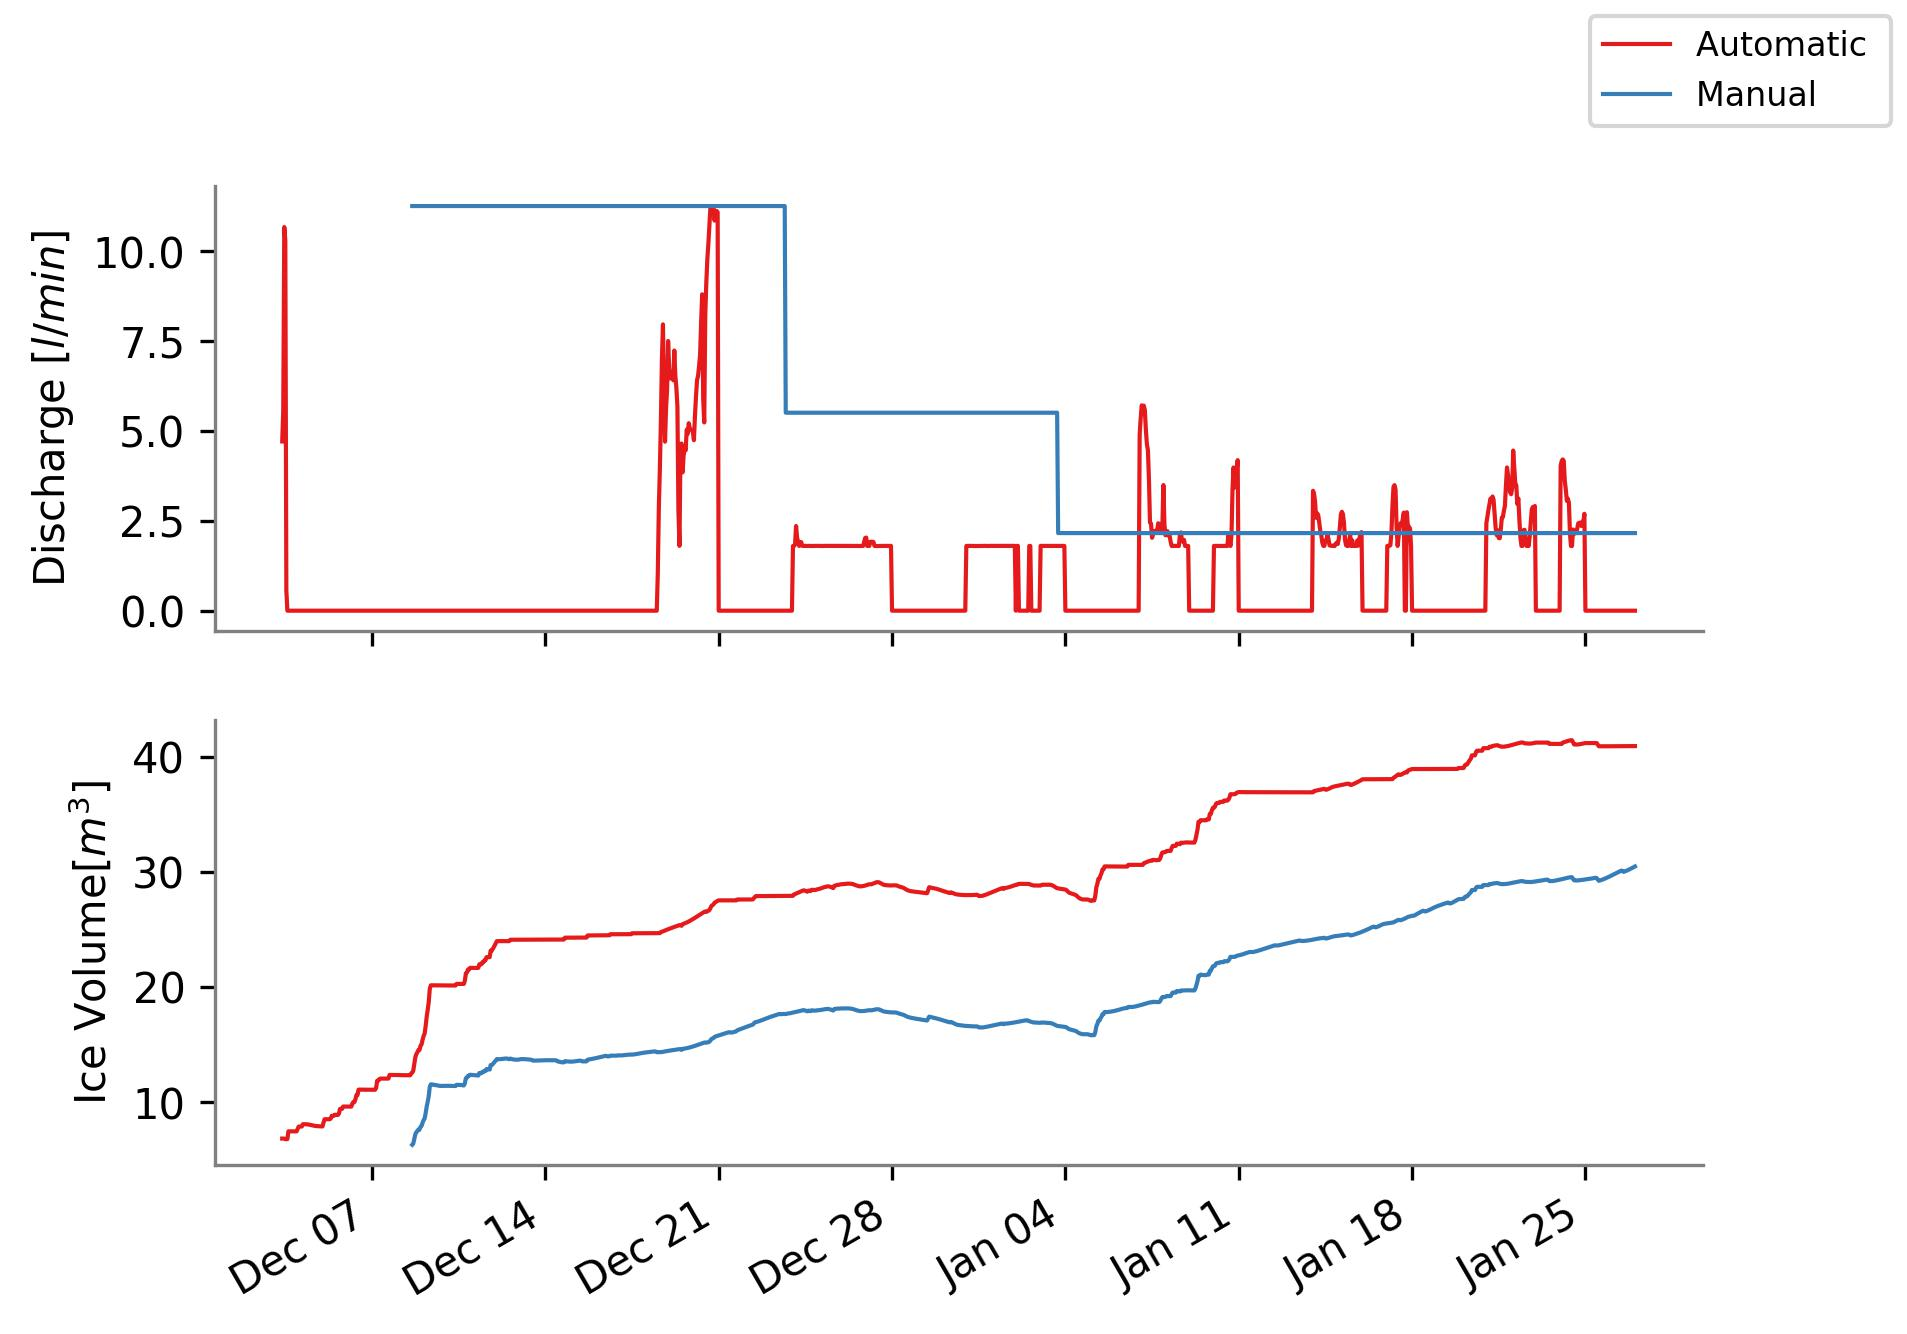
\includegraphics[width=\linewidth]{Figures/autovsmanual.jpg}
	\end{center}
	\caption{Icestupa in Ladakh, India on March 2017 was 24 $m$ tall and contained around 3700 $m^3$
		of water. Picture Credits: Lobzang Dadul}
	\label{fig:old_icestupa}
\end{figure}

\subsection{Validation}

\section{Discussion}

\section{Conclusions}

\section{Appendix}

\bibliographystyle{frontiersinSCNS_ENG_HUMS} \bibliography{references}

\end{document}
